\begin{figure*}[t]
\centering
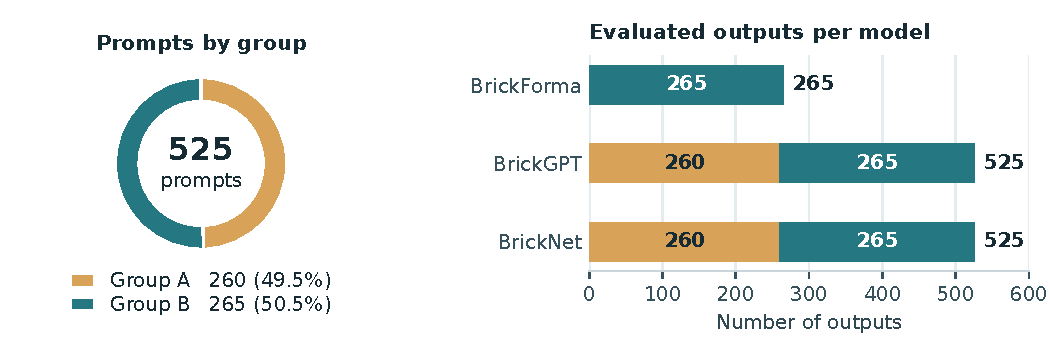
\includegraphics[width=\textwidth]{figures/comparison_20261116/01-cohorts.pdf}
\caption{Composition of the November 16 evaluation. Group A contains 260 shared prompts for BrickGPT and BrickNet. Group B contains 265 shared prompts for all three systems. The evaluation covers 525 distinct prompts and 1,315 exports.}
\label{fig:comparison-cohorts}
\end{figure*}

\begin{figure*}[t]
\centering
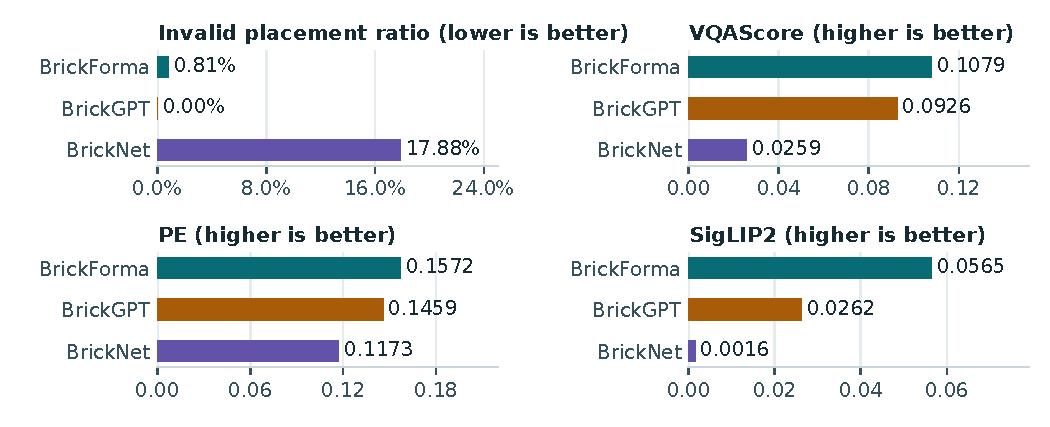
\includegraphics[width=\textwidth]{figures/comparison_20261116/02-means.pdf}
\caption{Mean scores on the 265 Group B prompts. Each mean assigns equal weight to each prompt. The plotted values correspond to Table~\ref{tab:main}.}
\label{fig:comparison-means}
\end{figure*}

\begin{figure*}[t]
\centering
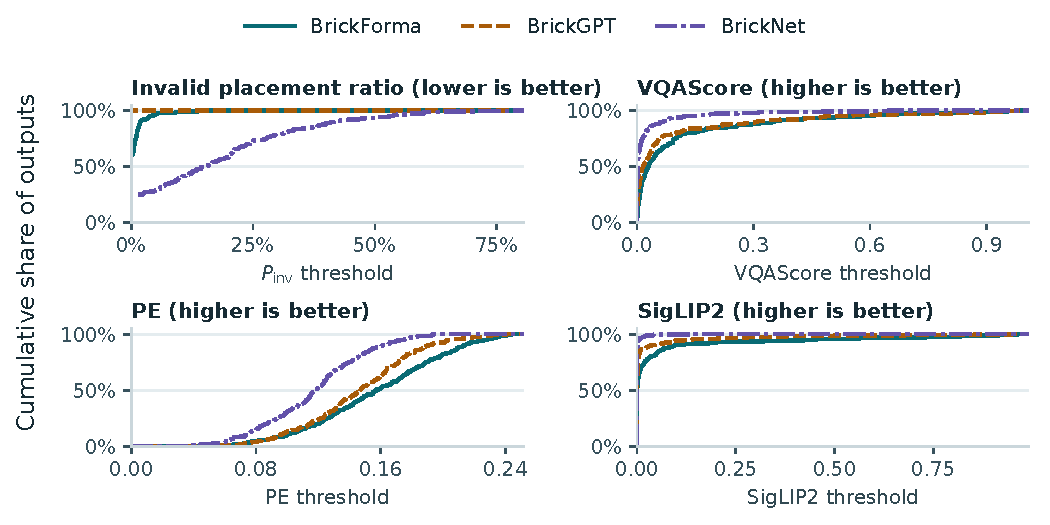
\includegraphics[width=\textwidth]{figures/comparison_20261116/03-distributions.pdf}
\caption{Empirical cumulative distributions of the four Group B scores. Each curve gives the fraction of a system's 265 outputs at or below the threshold on the horizontal axis.}
\label{fig:comparison-distributions}
\end{figure*}

\begin{figure*}[t]
\centering
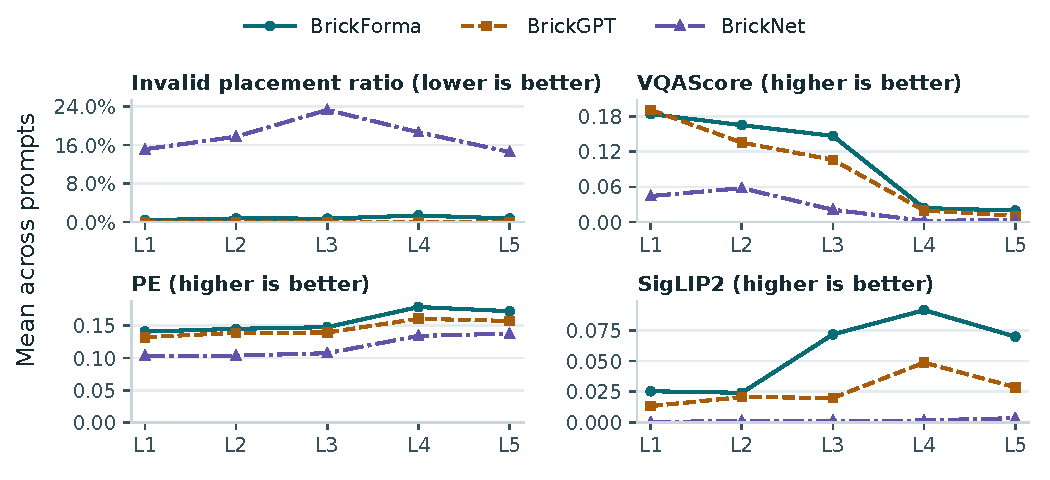
\includegraphics[width=\textwidth]{figures/comparison_20261116/04-by-level.pdf}
\caption{Group B mean scores by description level. Each point averages 53 prompts shared by all three systems. The plotted values correspond to Table~\ref{tab:levels}.}
\label{fig:comparison-levels}
\end{figure*}
